\documentclass[journal,transmag,times]{IEEEtran}

% *** GRAPHICS RELATED PACKAGES ***
\usepackage{graphicx}
\usepackage{pgfplots}
\usepackage{float}
\usepackage{caption}
\usepackage{subcaption}

% *** MATH PACKAGES ***
\usepackage{amsmath}
\usepackage{amssymb}
\usepackage{bm}
\usepackage{amsthm}

% *** SPECIALIZED LIST PACKAGES ***
\usepackage{algorithm,algpseudocode}
\renewcommand\algorithmicdo{until convergence}
\renewcommand\algorithmicfor{For}
\algtext*{EndFor}

% *** ALIGNMENT PACKAGES ***
\usepackage{array}

% *** PDF, URL AND HYPERLINK PACKAGES ***
\usepackage{url}

% *** TABLES PACKAGES ***
\usepackage{booktabs}

% *** BIBLIOGRAPHY PACKAGES ***
\usepackage[numbers]{natbib}

\begin{document}

\title{Anomaly Detection in Wireless Sensor Networks via Support Vector Data Description with Bayesian Optimization of Hyperparameters}

\author{
Van Vuong~Trinh$^1$,
Kim Phuc~Tran$^1$ and 
Anh Tuan~Mai$^2$\\
$^1$Division of Artificial Intelligence, Dong A University, Danang, Vietnam\\
$^2$International Training Institute for Materials Science (ITIMS),\\Hanoi University of Science and Technology, Hanoi, Vietnam\\
email: vanvuong.trinh@gmail.com
}

\markboth{Vietnam International Conference and Exhibition on Control and Automation}{VCCA-2017}

\maketitle

\section{Introduction}

\section{Support Vector Data Description and Preliminaries}

In this section, we briefly recall the support vector data sescription (SVDD) originally derived in \cite{Tax2004} which is an alternative of the known one-class support vector machines (OCSVM) \cite{Scholkopf2000} and analogous to support vector machines (SVM) \cite{Vapnik1998}.

\subsection{Theory}

We have a training data set $\{ \mathbf{x}_i \}$, $i=1,\dots,l$ for which we want to obtain a hypersphere with minimum volume, containing all (or most of) the data points. This is very sensitive to the most outliers in the training set. When one or a few very remote data points are in the training set, a very large hypersphere is obtained which will not represent the data approximately accurate. Therefore, we allow for some data points outside the hypersphere by introducing slack variables $\xi_i \ge 0$. Let $a$ and $R$ being reserved for the center and the radius of the hypersphere, the following primal optimization problem is considered:
\begin{subequations}\label{eq:svdd_primal_sphere}
\begin{align}
\underset{
	\begin{array}{c}
		 R, a, \xi_i
	\end{array}}{\text{Minimize }} & R^2 + C \sum_{i=1}^l \xi_i \\
\text{Subject to } & \left|\left| x_i - a \right|\right|^2 \le R^2 + \xi_i, \thinspace \xi_i \ge 0 \quad \forall i
\end{align}
\end{subequations}
where the parameter $C$ control the trade-o€ff between the volume and errors (number of normal data rejected).

In order to extend description capability,

In the feature space $\phi$, the primal problem changes into
\begin{subequations}\label{eq:svdd_primal}
\begin{align}
\underset{
	\begin{array}{c}
		 R, a, \xi_i
	\end{array}}{\text{Minimize }} & R^2 + C \sum_{i=1}^l \xi_i \\
\text{Subject to } & \left|\left| \phi \left(x_i\right) - \phi \left( a \right) \right|\right|^2 \le R^2 + \xi_i, \thinspace \xi_i \ge 0 \thinspace \forall i
\end{align}
\end{subequations}

\begin{align}
K \left( x_i, x_j \right) = \phi \left( x_i \right) \cdot \phi \left( x_j \right)
\end{align}

This leads to the dual optimization problem, which is a standard quadratic program (QP), as follows.
\begin{subequations}\label{eq:svdd_dual}
\begin{align}
\underset{
	\begin{array}{c}
		 \alpha_i
	\end{array}}{\text{Maximize }} & \sum_{i=1}^l \alpha_i K \left( x_i, x_i \right) - \sum_{i=1}^l \sum_{j=1}^l \alpha_i \alpha_j K \left( x_i, x_j \right)\\
\text{Subject to } & \sum_{i=1}^l \alpha_i = 1, \thinspace 0 \le \alpha_i \le C \thinspace \forall i
\end{align}
\end{subequations}
Such an optimisation is feasible if and only if the regularization parameter satisfies the inequality $C \ge 1{}/l$ with the optimal solution denoted as $\alpha^\star_k$. 

The data points corresponding to $\alpha^\star_k > 0$ are consequently referred to as the \emph{support vectors}. These support vectors characterize the scope of the description.

\subsection{Discriminant Function}

The image of the sphere center is
\begin{align}
\phi \left( a \right) = \sum_{i=1}^l \alpha^\star_i \phi \left( x_i \right)
\end{align}

By definition, the radius $R$ of the hypersphere is the kernel-based distance from the center $a$ to any of the support vectors on the boundary of the hypersphere, i.e. one correponds to $0< \alpha^\star_k < C$. Hence, the hypersphere radius $R$ is determined as:
\begin{align}
R^2 &= \left|\left| \phi \left( x_k \right) - \phi \left( a \right) \right|\right|^2 \nonumber \\
&= K \left( x_k, x_k \right) - 2 \sum_{i=1}^l \alpha^\star_i K \left( x_i, x_k \right)  
\\
&\quad + \sum_{i=1}^l \sum_{j=1}^l \alpha^\star_i \alpha^\star_j K \left( x_i, x_j \right) \nonumber
\end{align}
for any support vector $x_k$ that has $0 < \alpha^\star_k < C$.

Whether a data point $z$ is normal or not is in accordance to the kernel-based distance to the center of the sphere.
\begin{align}
R^2 - \left|\left| \phi \left( z \right) - \phi \left( a \right) \right|\right|^2 = 2 \sum_k \alpha^\star_k K \left( z, x_k \right) + v
\end{align}
where
\begin{align}
v = 2 \sum_{i=1}^l \sum_{j=1}^l \alpha^\star_i \alpha^\star_j K \left( x_i, x_j \right) + 1 - R^2
\end{align}

\subsection{Evaluation Measures via Geometric Mean Analysis}

While training a SVDD does not require the availability of abnormal data, its evaluation does. 

\begin{align}
g = \sqrt{Acc^+ \cdot Acc^-}
\end{align}

\section{Anomaly Detection Method for Wireless Sensor Networks using LOF and SVDD}

\subsection{Description of Aproach}

\subsection{Local Outlier Factor}



\subsection{Bayesian Optimization for Hyperparameter Selection}

Similar to other kernel methods, the performance of SVDD models is strongly affected by the kernel parameters.

\section{Simulation Results}

\cite{Suthaharan2010}

\subsection{Intel Berkeley Research Laboratory Data}

We consider a data set gathered from a wireless sensor network deployment at the Intel Berkeley Research Laboratory (IBRL) \cite{Buonadonna2005}. A wireless sensor network consisting of $54$ \emph{Mica2Dot} sensor nodes was deployed in the IBRL for a $30$ day ($720$ hour) period between 28th Feb 2004 and 5th April 2004 [10]. Figure~\ref{fig:ibrl_wsn} shows the deployed node locations in the laboratory. The sensors collect five measurements: light in Lux, temperature in degrees celsius, humidity (temperature corrected relative humidity) ranging from $0\%$ to $100\%$, voltage in volts and network topology information in each $30$ second interval. Node $0$ is the gateway node. Other nodes transmit their data in multiple hops to the gateway node. The furthest node in the network is about $10$ hops away from the gateway node. During the $30$ day period, the $54$ nodes collected about $2.3$ million readings.

\begin{figure}[H]
\centering
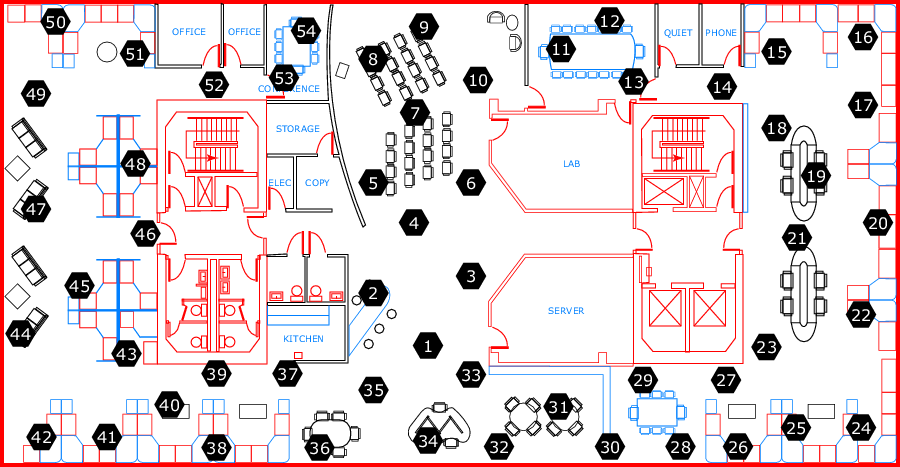
\includegraphics[scale=.25]{Pictures/ibrl_wsn}
\caption{A map of IBRL, with mote locations labeled in black.}
\label{fig:ibrl_wsn}
\end{figure}

In this paper we consider the IBRL data set obtained from $54$ nodes, namely node IDs from $1$ to $54$, during the first $10$ days period collected on March 2004. While the lab in Figure~\ref{fig:ibrl_wsn} has a total of $55$ sensors (including the gateway node), only $54$ of them provided data during the $10$ days time window examined in this paper. Also, only two features, namely temperature and humidity, are taken into account. However, since node $M_5$ did not contain any humidity data during this time window, we only 

It is notable that the notes contain a number of outliers.

Nodes $15$ and $18$ provided unrealistic data during some time intervals, i.e. too high or too low.

\subsection{Numerical Analysis of Parameters Optimization Algorithm}

Platform: 2.6 GHz Intel(R) Core(TM) i7 and 16GB of RAM.

Primal solution of SVDD is obtained using ILOG CPLEX 12.7.0.

NLopt nonlinear optimization package \cite{nlopt}

\section{Conclusion and Future Work}

\bibliographystyle{IEEEtran}
\bibliography{wsnbib,svmbib,ocsvmbib,ibrlbib,miscbib}

\end{document}


